\documentclass[../../include.tex]{subfiles}
\begin{document}
\begin{table}[ht]
	\caption{Report on the $L_1$ errors of the $\mathrm{S^1 IIOE}$(stabilized) and the $\mathrm{FLIIOE}$(flux limited) schemes for a smooth hump, $ \tau = h $.}
	\begin{center} \footnotesize
		\begin{tabular}{|c|c|c|c|c|}
		\hline
	 	& $ \mathrm{S^1 IIOE} $ &$ \mathrm{S^1 IIOE} $ &$ \mathrm{FLIIOE} $ & $ \mathrm{FLIIOE} $ \\
		$ n $ & $\mathrm{L_1 error}$ & EOC & $\mathrm{L_1 error}$ & EOC \\
		\hline
		\lower.3ex\hbox{40} &  \lower.3ex\hbox{9.82 $10^{-2}$} & & \lower.3ex\hbox{7.51 $10^{-2}$} &\\
		\hline
		\lower.3ex\hbox{80} &  \lower.3ex\hbox{3.38 $10^{-2}$} &\lower.3ex\hbox{1.54} & \lower.3ex\hbox{2.66 $10^{-2}$} &\lower.3ex\hbox{1.50}  \\
		\hline
		\lower.3ex\hbox{160} &  \lower.3ex\hbox{1.01 $10^{-2}$} &\lower.3ex\hbox{1.74}& \lower.3ex\hbox{7.55 $10^{-3}$} &\lower.3ex\hbox{1.82} \\
		\hline
		\lower.3ex\hbox{320} &  \lower.3ex\hbox{2.73 $10^{-3}$} &\lower.3ex\hbox{1.89}& \lower.3ex\hbox{1.96 $10^{-3}$} &\lower.3ex\hbox{1.95}\\
		\hline
		\lower.3ex\hbox{640} &  \lower.3ex\hbox{7.11 $10^{-4}$} &\lower.3ex\hbox{1.94}& \lower.3ex\hbox{5.22 $10^{-4}$} &\lower.3ex\hbox{1.91} \\
		\hline
		\lower.3ex\hbox{1280} &  \lower.3ex\hbox{1.83 $10^{-4}$} &\lower.3ex\hbox{1.96}& \lower.3ex\hbox{1.41 $10^{-4}$} &\lower.3ex\hbox{1.89} \\
		\hline
		\end{tabular}
	\end{center}
	\label{tab:siioe_hump}
\end{table}

\begin{figure}[h!]
	\centering
	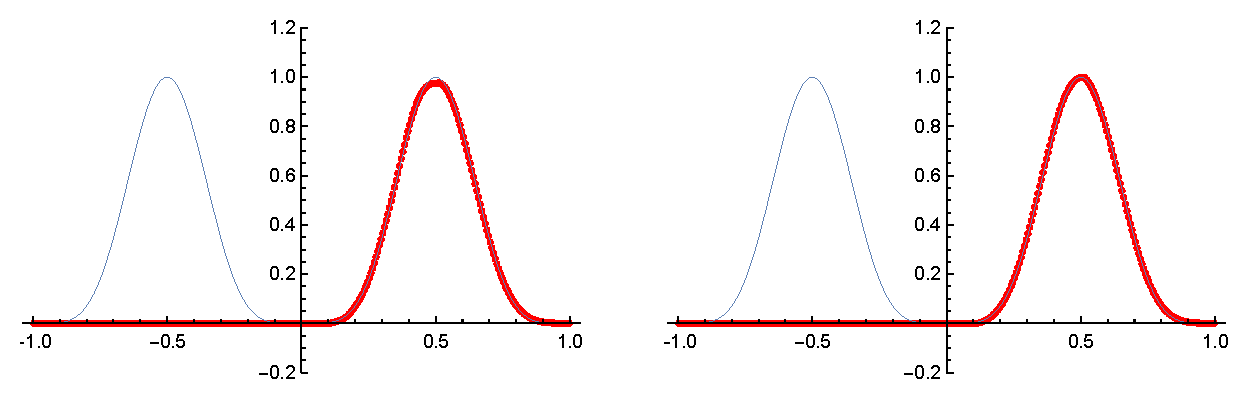
\includegraphics[width=\textwidth]{figures/compareHump.pdf}
	\caption{Comparing the $\mathrm{S^1 IIOE}$(stabilized) and the $\mathrm{FLIIOE}$(flux limited) schemes with the exact solution  in time $ t=1 $, $ n=320 $, $ \tau=h $.}
	\label{fig:compare_S1FL_hump}
\end{figure}

\begin{table}[ht]
	\caption{Report on the $L_1$ errors of the $\mathrm{S^1 IIOE}$(stabilized) and the $\mathrm{FLIIOE}$(flux limited) schemes for a discontinous piecewise profile, $ \tau = h $.}
	\begin{center} \footnotesize
		\begin{tabular}{|c|c|c|c|c|}
			\hline
			& $ \mathrm{S^1 IIOE} $ &$ \mathrm{S^1 IIOE} $ &$ \mathrm{FLIIOE} $ & $ \mathrm{FLIIOE} $ \\
			$ n $ & $\mathrm{L_1 error}$ & EOC & $\mathrm{L_1 error}$ & EOC \\
			\hline
			\lower.3ex\hbox{40} &  \lower.3ex\hbox{2.03 $10^{-1}$} & & \lower.3ex\hbox{1.49 $10^{-1}$}&\\
			\hline
			\lower.3ex\hbox{80} &  \lower.3ex\hbox{1.31 $10^{-1}$} &\lower.3ex\hbox{0.63}& \lower.3ex\hbox{9.4 $10^{-2}$} & \lower.3ex\hbox{0.66}\\
			\hline
			\lower.3ex\hbox{160} &  \lower.3ex\hbox{8.38 $10^{-2}$} &\lower.3ex\hbox{0.64}& \lower.3ex\hbox{5.91 $10^{-2}$} &\lower.3ex\hbox{0.67}\\
			\hline
			\lower.3ex\hbox{320} &  \lower.3ex\hbox{5.35 $10^{-2}$} &\lower.3ex\hbox{0.65}& \lower.3ex\hbox{3.72 $10^{-2}$} &\lower.3ex\hbox{0.67} \\
			\hline
			\lower.3ex\hbox{640} &  \lower.3ex\hbox{3.41 $10^{-2}$} &\lower.3ex\hbox{0.65}& \lower.3ex\hbox{2.35 $10^{-2}$} &\lower.3ex\hbox{0.66}\\
			\hline
			\lower.3ex\hbox{1280} &  \lower.3ex\hbox{2.16 $10^{-2}$} &\lower.3ex\hbox{0.66}& \lower.3ex\hbox{1.48 $10^{-2}$} &\lower.3ex\hbox{0.67}\\
			\hline
		\end{tabular}
	\end{center}
	\label{tab:siioe_disc}
\end{table}

\begin{figure}[h!]
	\centering
	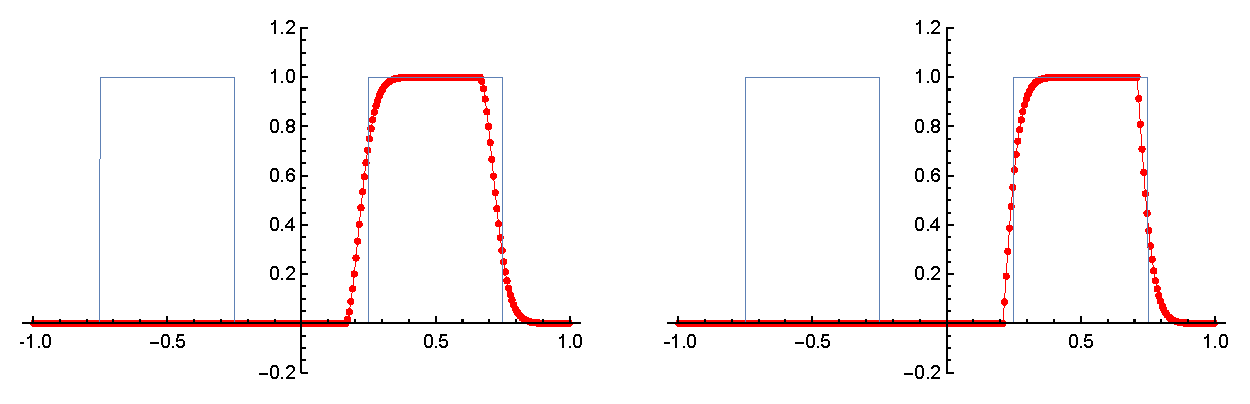
\includegraphics[width=\textwidth]{figures/compareDisc.pdf}
	\caption{Comparing the $\mathrm{S^1 IIOE}$(stabilized) and the $\mathrm{FLIIOE}$(flux limited) schemes with the exact solution  in time $ t=1 $, $ n=320 $, $ \tau=h $.}
	\label{fig:compare_S1FL_disc}
\end{figure}

\begin{table}[ht]
	\caption{Report on the $L_1$ errors of the $\mathrm{FLIIOE}$(flux limited) scheme for a shock solution of the inviscid Burgers' equation, $ \tau = h $.}
	\begin{center} \footnotesize
		\begin{tabular}{|c|c|c|}
			\hline
			 &$ \mathrm{FLIIOE} $ & $ \mathrm{FLIIOE} $ \\
			$ n $ &  $\mathrm{L_1 error}$ & EOC \\
			\hline
			\lower.3ex\hbox{100} & \lower.3ex\hbox{2.46 $10^{-3}$} & \\
			\hline
			\lower.3ex\hbox{200} &  \lower.3ex\hbox{1.24 $10^{-3}$} &\lower.3ex\hbox{1.00} \\
			\hline
			\lower.3ex\hbox{400} &  \lower.3ex\hbox{6.18 $10^{-4}$}  &\lower.3ex\hbox{1.00}\\
			\hline
		\end{tabular}
	\end{center}
	\label{tab:fliioe_shock}
\end{table}
\begin{table}[ht]
	\caption{Report on the $L_1$ errors of the $\mathrm{FLIIOE}$(flux limited) scheme for a rarefaction wave-solution of the inviscid Burgers' equation, $ \tau = h $.}
	\begin{center} \footnotesize
		\begin{tabular}{|c|c|c|}
			\hline
			&$ \mathrm{FLIIOE} $ & $ \mathrm{FLIIOE} $ \\
			$ n $ &  $\mathrm{L_1 error}$ & EOC \\
			\hline
			\lower.3ex\hbox{100} & \lower.3ex\hbox{3.10 $10^{-3}$} & \\
			\hline
			\lower.3ex\hbox{200} &  \lower.3ex\hbox{1.64 $10^{-3}$} &\lower.3ex\hbox{0.92} \\
			\hline
			\lower.3ex\hbox{400} &  \lower.3ex\hbox{8.48 $10^{-4}$}  &\lower.3ex\hbox{0.95}\\
			\hline
		\end{tabular}
	\end{center}
	\label{tab:fliioe_rare}
\end{table}
\begin{figure}[h!]
	\centering
	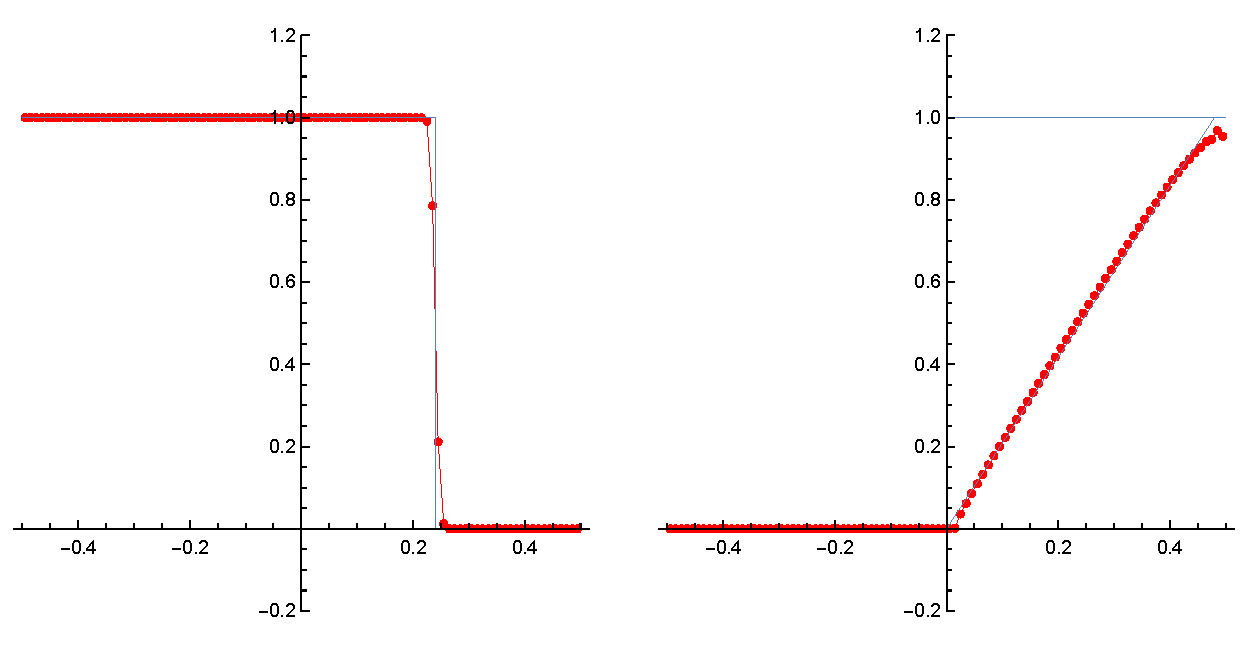
\includegraphics[width=\textwidth]{figures/shockRare.pdf}
	\caption{Comparing the $\mathrm{FLIIOE}$(flux limited) schemes with the exact solution in time $ t=0.48 $, $ n=100 $, $ \tau=h $.}
	\label{fig:fliioe_shock_rare}
\end{figure}
\end{document}